\section{Additional Figures}
\label{app:additional-figures}

The main text uses only the figures that directly support the narrative spine of
the paper. The supplementary material contains a somewhat richer figure set under
`outputs/figures/`, including intermediate mechanism schematics and witness
renderings. These assets are part of the reproducibility
record and can be promoted into the main text later if venue constraints allow.

\subsection*{Deletion Cases}

\begin{figure}[h]
    \centering
    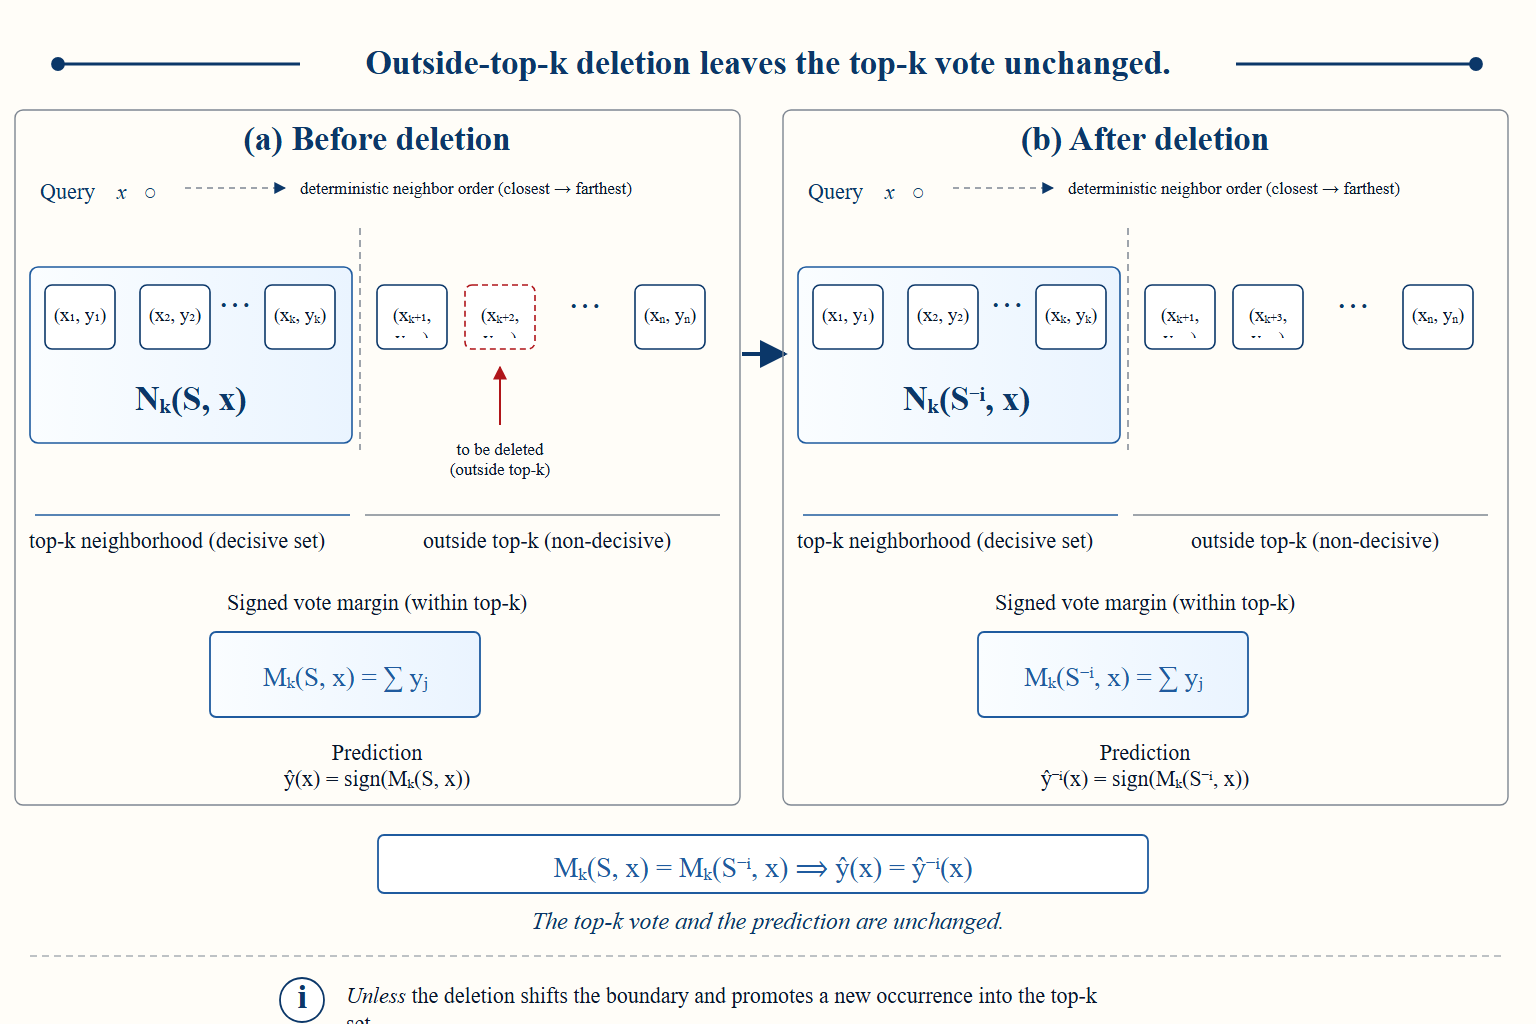
\includegraphics[width=0.82\linewidth]{outputs/figures/recreated_fig05.png}
    \caption{Two cases for deletion. Case A (left): deleting an occurrence outside
    the ordered top-$k$ neighborhood is inert; the top-$k$ set and margin are
    unchanged. Case B (right): deleting an occurrence inside the top-$k$ set may
    promote the rank-$(k+1)$ occurrence into the vote, changing the margin.}
    \label{fig:stable-deletion}
\end{figure}

\subsection*{Replace-One Flip Mechanisms}

\begin{figure}[h]
    \centering
    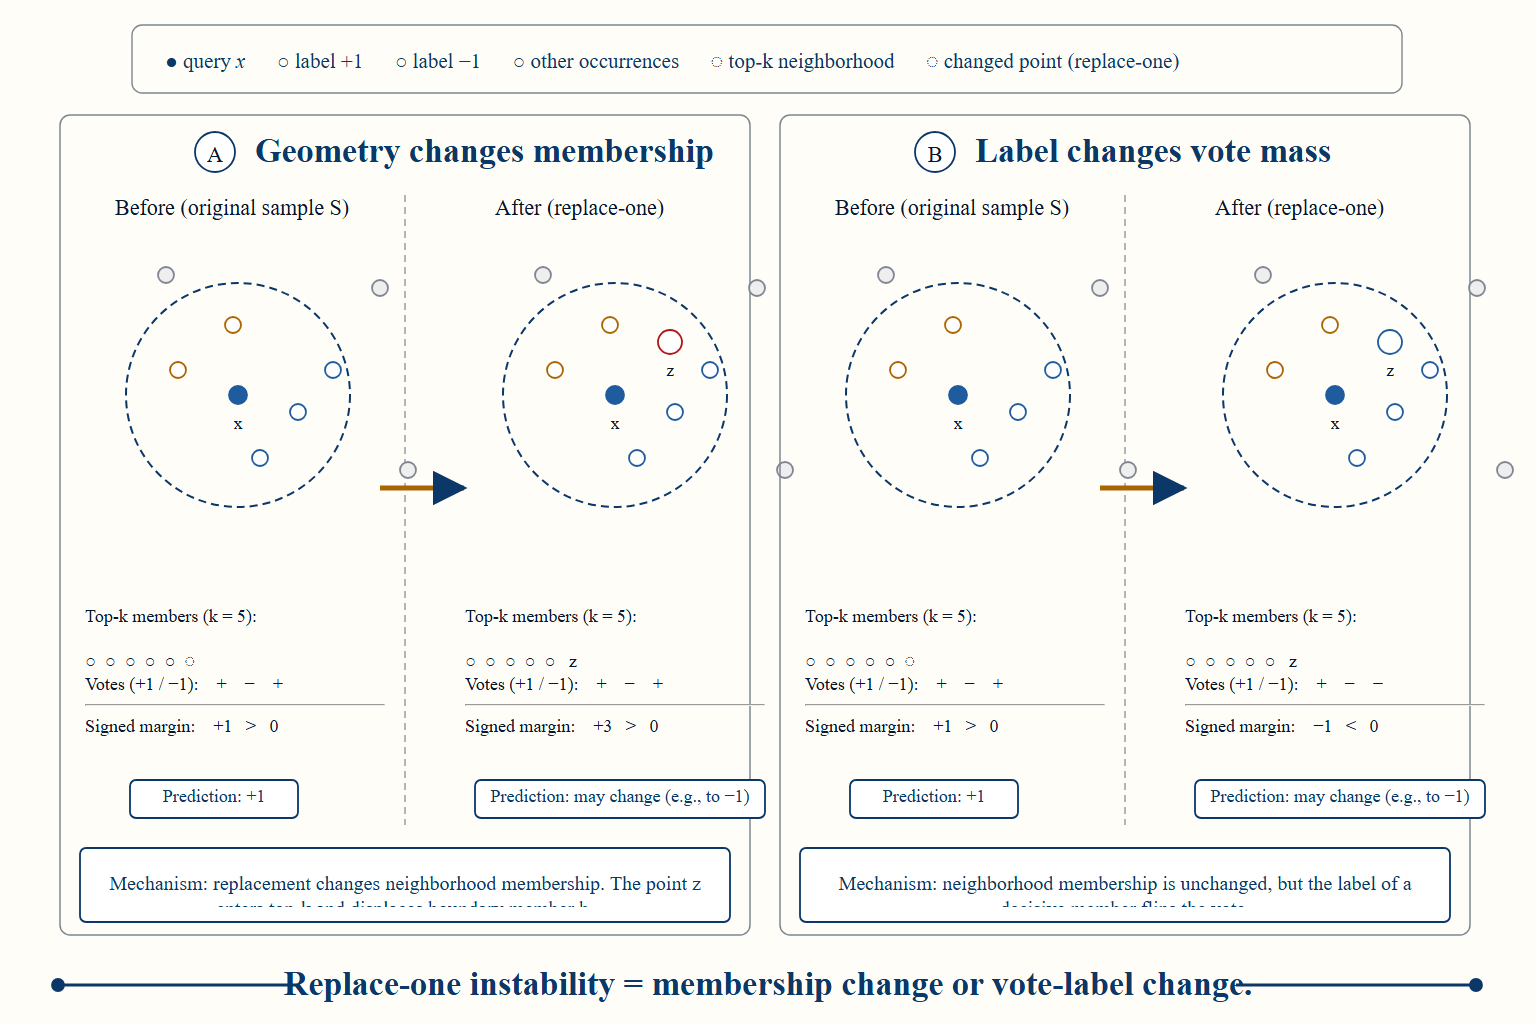
\includegraphics[width=0.82\linewidth]{outputs/figures/recreated_fig07.png}
    \caption{Replace-one perturbations can flip the decision either by moving a
    new occurrence into the decisive neighborhood or by changing the label
    composition of a neighborhood that was already geometrically close to the
    boundary.}
    \label{fig:replace-flip}
\end{figure}

\subsection*{Tie-Breaking Effects}

\begin{figure}[h]
    \centering
    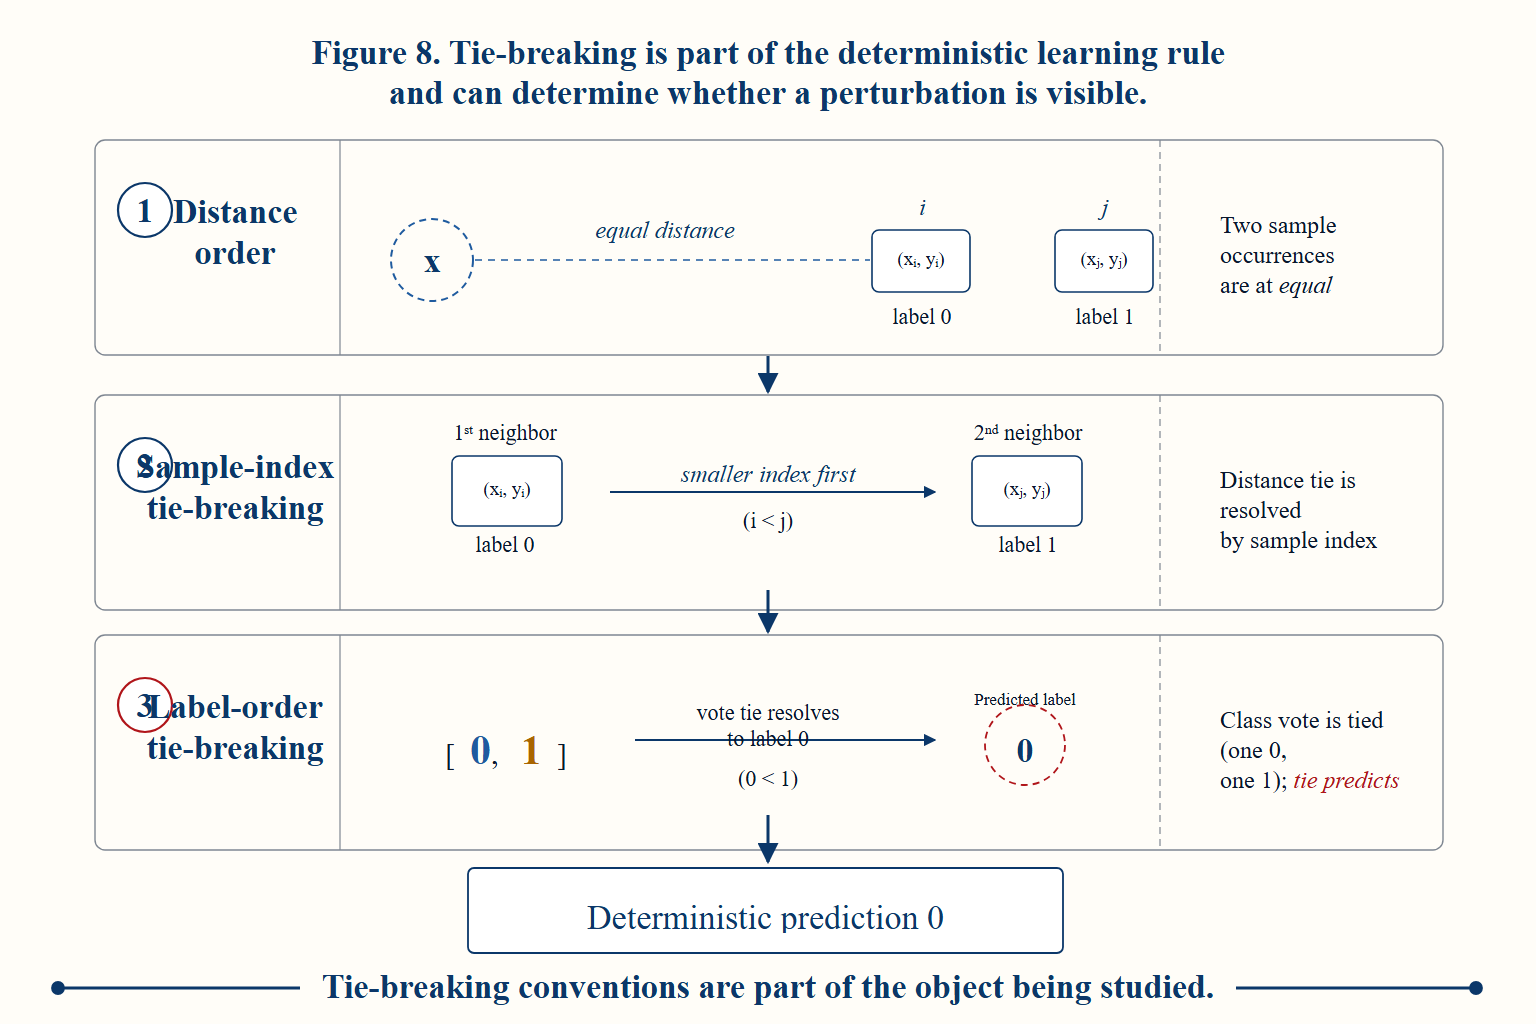
\includegraphics[width=0.82\linewidth]{outputs/figures/recreated_fig08.png}
    \caption{Tie-breaking is not decorative. When several occurrences are at
    equal distance, the deterministic sample order and fixed label order can
    determine whether a perturbation is visible to the predictor.}
    \label{fig:tie-microscope}
\end{figure}

